 \documentclass{beamer}
%\documentclass[handout]{beamer}
\usetheme{metropolis}

%\setbeameroption{show notes}
%\setbeameroption{show notes on second screen}

% Packages
\usepackage[utf8]{inputenc}

\usepackage{animate}

\usepackage{appendixnumberbeamer}
\usepackage{xcolor}
\usepackage{multirow}
% Maths
\usepackage{amsthm}
\usepackage{tikz}
\usetikzlibrary{cd}

% References
\usepackage{biblatex}
\addbibresource{./references.bib}

% Package Settings
% AMSTHM
\theoremstyle{plain}
\newtheorem{thm}{Theorem}[section]
\newtheorem{mylemma}[thm]{Lemma}
\newtheorem{cor}[thm]{Corollary}
\newtheorem{rem}[thm]{Remark}
\newtheorem{alg}[thm]{Algorithm}

\theoremstyle{definition}
\newtheorem{defn}[thm]{Definition}

\newcommand{\TODO}[1]{{\color{red}*** #1 ***}}

\renewcommand{\phi}{\varphi}

% BEAMER
% Hack for only and tabular
\newcommand{\tabularonly}{AS}
% Hack for tilde and hat
\newcommand{\mytilde}[1]    {\ensuremath{\tilde{#1}}}
\newcommand{\myhat}[1]    {\ensuremath{\widehat{#1}}}
% Hack to display \Gamma with a little bit of space to the left
% Otherwise \ind _ \Gamma ^ H looks really weird
\let\oldGamma\Gamma
\renewcommand{\Gamma}{{\hspace{0.5pt} \oldGamma}}
% Hack to reference the notation-definition in "lift a.s. normaliser"
\newcommand{\refdef}    {{(6.1)}}

% Symbols
% Write function definitions like
% f \from A \to B
\newcommand{\from}	{\ensuremath{\colon}}
\renewcommand{\to}	{\ensuremath{\rightarrow}}
\newcommand{\into}	{\ensuremath{\hookrightarrow}}
\newcommand{\onto}	{\ensuremath{\twoheadrightarrow}}
\newcommand{\iso}	{\ensuremath{\xrightarrow{\,\raisebox{-1pt}{\ensuremath{\scriptstyle{\sim}}}\,}}}
\newcommand{\N}	{\ensuremath{\mathbb N}}
\newcommand{\Z}	{\ensuremath{\mathbb Z}}
\newcommand{\Q}	{\ensuremath{\mathbb Q}}
\newcommand{\Sn}{{\ensuremath{\mathrm{S}_n}}}
\newcommand{\uln} {{\ensuremath{\underline n}}}

%%% Categories
\newcommand{\permgrp}   {\ensuremath{\mathbf{PermGrp}}}

%%% Unary Operators
% Functions
\DeclareMathOperator{\dom}{dom}
\DeclareMathOperator{\id}{id}
\DeclareMathOperator{\im}{Im}
% Groups
\DeclareMathOperator{\sym}{Sym}
\DeclareMathOperator{\Sym}{Sym}
\DeclareMathOperator{\alternating}{Alt}
\DeclareMathOperator{\Alt}{Alt}
\DeclareMathOperator{\soc}{soc}
\DeclareMathOperator{\aut}{Aut}
\DeclareMathOperator{\Aut}{Aut}
\DeclareMathOperator{\out}{Out}
\DeclareMathOperator{\Out}{Out}
\DeclareMathOperator{\ind}{Ind}
\DeclareMathOperator{\res}{Res}
\DeclareMathOperator{\stab}{Stab}
\newcommand{\hatOperator}   {\ensuremath{\, \myhat \cdot\,}}
\def\Norm#1#2{\mathrm{N}_{#1}(#2)}

%%% Binary Operators %%%
\newcommand{\union}{\mathbin{\cup}}
\newcommand{\bigunion}{\mathbin{\bigcup}}
\newcommand{\disjointunion}{\mathbin{\uplus}}
\newcommand{\intersection}{\mathbin{\cap}}
\newcommand{\bigintersection}{\mathbin{\bigcap}}
\newcommand{\norm}{\mathbin{\lhd}}
\newcommand{\characteristic}{\mathbin{\text{char}}}


% New commands
\newcommand{\abs}[1]	{%
	\ensuremath{
		\left| #1 \right|
	}%
}
\newcommand{\gen}[1]	{
	\ensuremath{
		\left\langle \, #1 \, \right\rangle
	}
}
\newcommand{\set}[1]	{
	\ensuremath{
		\left\{ #1 \right\}
	}
}
\newcommand{\sset}[2] {
	\ensuremath{
		\left\{ \left.\,
			#1
		~\right|~
			#2
		\,\right\}
	}
}


\title{Towards Efficient Normalizers For Primitive Groups}
\date{July 15th, 2020}
\author{Sergio Siccha}
\institute{TU Kaiserslautern}

\begin{document}

\maketitle
\note{
VERSION WITH NOTES!
}

\begin{frame}[plain, noframenumbering]{Overview}
\begin{itemize}
\setlength{\itemsep}{\fill}
\item \TODO{}
\item \TODO{}
\end{itemize}
\end{frame}

\section{Introduction}
\begin{frame}{Normalizers}

Let $G, M \leq K$ be groups.
The \emph{normalizer of $G$ in $M$} is
the group
\[
N_M(G) = \set{ m \in M ~|~ G ^ m = G }.
\]
\vspace{0.5em}

\pause
\begin{block}{Theorem (D. Wiebking \cite{wiebking:normalizers-simply-exponential})}
Let $G = \gen X \leq \Sym \Omega$.
A generating set of $N_{\Sym \Omega}$
can be computed in time $\gen X 2 ^ {O(\abs \Omega)}$.
\end{block}
\end{frame}

\note{
theoretical,
canonical labelling
}

\begin{frame}{Theory and Practice}

Let $G = \gen X \leq \Sym \Omega$, and $n := \abs \Omega$.
We consider
\begin{itemize}
\item deterministic polynomial time $O(\abs X n ^ c)$
\item Las Vegas nearly-linear time $O(\abs X n \, (\log n) ^ c)$
\end{itemize}
\vspace{1em}

\pause
We can compute in polynomial and in nearly-linear time:
\begin{itemize}
\item the order $\abs G$
\item a composition series of $G$
\item the socle of $G$
\item \ldots
\end{itemize}
\end{frame}

\begin{frame}{Primitive Groups}
A transitive group $G \leq \Sym \Omega$ is
\emph{imprimitive}, if there exists a non-trivial $G$-invariant partition of
$\Omega$,
otherwise it is \emph{primitive}.

\begin{columns}
\begin{column}{0.5\textwidth}
$D_8 := \gen{ (1,2,3,4),\, (1,4)(2,3) }$
\\[1em]

\only<1>{\vspace{1\baselineskip}}
\only<2->{
$\set{ \set{1,3}, \set{2,4} }$ is $D_8$-invariant.
}
\end{column}
\begin{column}{0.3\textwidth}
{
\only<1->{
\begin{figure}[h]
\centering
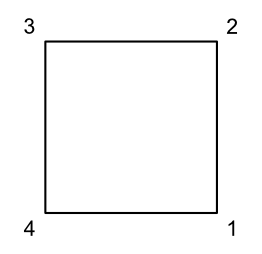
\includegraphics[width=0.9\textwidth]{./pictures/square.png}
\caption{A square}
\end{figure}
}
}
\end{column}
\end{columns}
\end{frame}

\begin{frame}%{Resultat}
\begin{block}{Theorem (S.)}
Let $G = \gen X \leq \Sym \Omega$ be a primitive group
with non-regular socle.
We can compute (a generating set of) $N_{\Sym \Omega}(G)$
in time $O(\abs X \abs \Omega ^ c)$.
\end{block}
\vspace{1em}
Note: Most parts in nearly-linear time.

\vspace{1em}
\pause
Note: For $M \leq \sym \Omega$ we have
$N_{M}(G) = M \cap N_{\sym \Omega}(G)$.
\end{frame}

\begin{frame}{Implementation}
A partial implementation is available at the github repository
\begin{center}
\href{https://github.com/ssiccha/NormalizersOfPrimitiveGroups}{ssiccha/NormalizersOfPrimitiveGroups}
\end{center}
\end{frame}


\section{Strategy}
\begin{frame}{Standing on the shoulders of giants}
The algorithm depends heavily on
\begin{itemize}
\item the O'Nan-Scott Theorem
\item the classification of finite simple groups (CFSG)
\end{itemize}
\end{frame}

\begin{frame}{Classification of primitive groups}
Let $G$ be a group. The \emph{socle} of $G$, denoted $\soc G$,
is the group generated by all minimal normal subgroups of $G$.
\\[1em]

\begin{block}{O'Nan-Scott Theorem}
    Let $G \leq \sym \Omega$ be primitive.
    We know all possible permutational isomorphism types of
    \pause
    \vspace{-0.5em}
    \begin{itemize}
        \item
        $\soc G$,
        \item
        $N_{\sym \Omega}(\soc G)$.
    \end{itemize}
\end{block}

$N_{\sym \Omega}(\soc G)$ is closely related to
\emph{product action wreath products}.
\end{frame}

\begin{frame}{Wreath products}
\begin{defn}
    Let $H$ be a group and let $K \leq S_\ell$.
    $K$ acts on $H ^ \ell$ by permuting components.
    The group
    $H \wr K := H ^ \ell \rtimes K$
    is the \emph{wreath product of $H$ with $K$}.
\end{defn}

\pause
If $H \leq \Sym \Delta$, then $H \wr K$ acts faithfully on
\begin{itemize}
\item $\Delta \times \set{1, \ldots, \ell}$ via the \emph{imprimitive action}
\item $\Delta ^ \ell$ via the \emph{product action}
\end{itemize}

Where $i$-th copy of $H$ acts on $i$-th copy of $\Delta$, $K$ permutes the copies.
\end{frame}

\note{
    Make sure to explain intuition behind wreath products
}

\begin{frame}{Socle}
The socle of a primitive group is characteristically simple.
\\[2em]
If $\soc G \cong T ^ \ell$ is non-regular, then
$G \into \Aut T \wr S_\ell$.
\end{frame}

\section{Permutation morphisms}

\section{Reduction homomorphism}
\begin{frame}
only say that
$\abs{\Out T} \leq ? \log_2 d$
and
$\ell = \log_d n$.
\end{frame}

\section{Implementation}

\begin{frame}[standout]
Thanks!
\end{frame}

\printbibliography
\appendix
\end{document}
